\begin{center}
    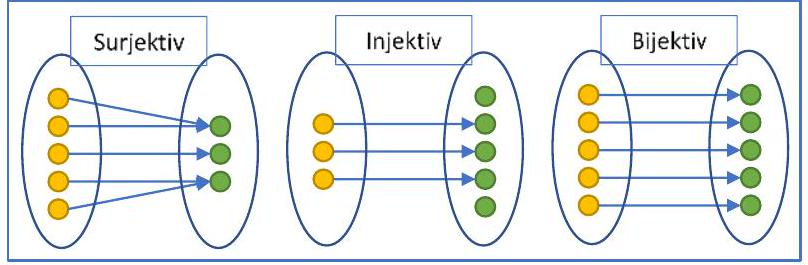
\includegraphics[scale=0.2]{Analysis1/zsf/Images/Stetige_Funktionen/2024_01_20_7bfda6c084929ccc01ffg-01(3).jpg}
\end{center}


\begin{definition}{Umkehrfunktion}
\begin{itemize}
  \item Bijektive Funktion $f: D \rightarrow W$
  \item Umkehrunktion $f^{-1} \quad g: W \rightarrow D$
\end{itemize}
Vorgehen $f(x)=y$:
\begin{itemize}
  \item Nach $x$ auflösen $\quad \rightarrow x=g(y)$
  \item Variablen vertauschen $\rightarrow y=g(x)$
\end{itemize}
\end{definition}



\begin{theorem}{Operationen von Funktionen}
    \begin{itemize}
  \item Addition $x \rightarrow f(x)+g(x)$
  \item Subtraktion $x \rightarrow f(x)-g(x)$
  \item Multiplikation $x \rightarrow f(x) \cdot g(x)$
    \item Division $x \rightarrow f(x) / g(x)$
\end{itemize}



\begin{itemize}
  \item Komposition/Verkettung: $(g \circ f)(x)=g(f(x))$
\end{itemize}
\end{theorem}

\begin{definition}{Symmetrie}
\begin{itemize}
  \item gerade $f(-x)=f(x)$
  \item ungerade $f(-x)=-f(x)$
\end{itemize}
\end{definition}

\begin{center}
    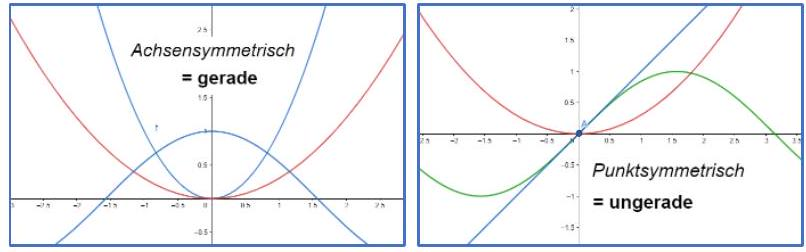
\includegraphics[scale=0.3]{Analysis1/zsf/Images/Stetige_Funktionen/2024_01_20_7bfda6c084929ccc01ffg-01(2).jpg}
\end{center}

\begin{definition}{Beschränktheit}
    Sei $f \in \R^D$.
    \begin{enumerate}
        \item $f$ ist \emph{nach oben beschränkt}, falls $f(D) \subseteq \R$ nach oben beschränkt.
        \item $f$ ist \emph{nach unten beschränkt}, falls $f(D) \subseteq \R$ nach unten beschränkt.
        \item $f$ ist \emph{beschränkt}, falls $f(D) \subseteq \R$ beschränkt.
    \end{enumerate}
\end{definition}

\begin{definition}{Monotonie}
    \begin{itemize}
  \item monoton wachsend $f\left(x_{1}\right) \leq f\left(x_{2}\right)$
  \item streng monoton wachsend $f\left(x_{1}\right)<f\left(x_{2}\right)$
  \item monoton fallend $f\left(x_{1}\right) \geq f\left(x_{2}\right)$
  \item streng monoton wachsend $f\left(x_{1}\right)>f\left(x_{2}\right)$
\end{itemize}
\end{definition}


